\documentclass[journal,12pt,twocolumn]{IEEEtran}

\usepackage{setspace}
\usepackage{gensymb}

\singlespacing


\usepackage[cmex10]{amsmath}

\usepackage{amsthm}

\usepackage{mathrsfs}
\usepackage{txfonts}
\usepackage{stfloats}
\usepackage{bm}
\usepackage{cite}
\usepackage{cases}
\usepackage{subfig}

\usepackage{longtable}
\usepackage{multirow}

\usepackage{enumitem}
\usepackage{mathtools}
\usepackage{steinmetz}
\usepackage{tikz}
\usepackage{circuitikz}
\usepackage{verbatim}
\usepackage{tfrupee}
\usepackage[breaklinks=true]{hyperref}
\usepackage{graphicx}
\usepackage{graphics}
\usepackage{tkz-euclide}
\usepackage{float}

\usetikzlibrary{calc,math}
\usepackage{listings}
    \usepackage{color}                                            %%
    \usepackage{array}                                            %%
    \usepackage{longtable}                                        %%
    \usepackage{calc}                                             %%
    \usepackage{multirow}                                         %%
    \usepackage{hhline}                                           %%
    \usepackage{ifthen}                                           %%
    \usepackage{lscape}     
\usepackage{multicol}
\usepackage{chngcntr}

\DeclareMathOperator*{\Res}{Res}

\renewcommand\thesection{\arabic{section}}
\renewcommand\thesubsection{\thesection.\arabic{subsection}}
\renewcommand\thesubsubsection{\thesubsection.\arabic{subsubsection}}

\renewcommand\thesectiondis{\arabic{section}}
\renewcommand\thesubsectiondis{\thesectiondis.\arabic{subsection}}
\renewcommand\thesubsubsectiondis{\thesubsectiondis.\arabic{subsubsection}}


\hyphenation{op-tical net-works semi-conduc-tor}
\def\inputGnumericTable{}                                 %%

\lstset{
%language=C,
frame=single, 
breaklines=true,
columns=fullflexible
}
\begin{document}


\newtheorem{theorem}{Theorem}[section]
\newtheorem{problem}{Problem}
\newtheorem{proposition}{Proposition}[section]
\newtheorem{lemma}{Lemma}[section]
\newtheorem{corollary}[theorem]{Corollary}
\newtheorem{example}{Example}[section]
\newtheorem{definition}[problem]{Definition}

\newcommand{\BEQA}{\begin{eqnarray}}
\newcommand{\EEQA}{\end{eqnarray}}
\newcommand{\define}{\stackrel{\triangle}{=}}
\newcommand\hlight[1]{\tikz[overlay, remember picture,baseline=-\the\dimexpr\fontdimen22\textfont2\relax]\node[rectangle,fill=blue!50,rounded corners,fill opacity = 0.2,draw,thick,text opacity =1] {$#1$};}
\bibliographystyle{IEEEtran}
\providecommand{\mbf}{\mathbf}
\providecommand{\pr}[1]{\ensuremath{\Pr\left(#1\right)}}
\providecommand{\qfunc}[1]{\ensuremath{Q\left(#1\right)}}
\providecommand{\sbrak}[1]{\ensuremath{{}\left[#1\right]}}
\providecommand{\lsbrak}[1]{\ensuremath{{}\left[#1\right.}}
\providecommand{\rsbrak}[1]{\ensuremath{{}\left.#1\right]}}
\providecommand{\brak}[1]{\ensuremath{\left(#1\right)}}
\providecommand{\lbrak}[1]{\ensuremath{\left(#1\right.}}
\providecommand{\rbrak}[1]{\ensuremath{\left.#1\right)}}
\providecommand{\cbrak}[1]{\ensuremath{\left\{#1\right\}}}
\providecommand{\lcbrak}[1]{\ensuremath{\left\{#1\right.}}
\providecommand{\rcbrak}[1]{\ensuremath{\left.#1\right\}}}
\theoremstyle{remark}
\newtheorem{rem}{Remark}
\newcommand{\sgn}{\mathop{\mathrm{sgn}}}
\providecommand{\abs}[1]{\left\vert#1\right\vert}
\providecommand{\res}[1]{\Res\displaylimits_{#1}} 
\providecommand{\norm}[1]{\left\lVert#1\right\rVert}
%\providecommand{\norm}[1]{\lVert#1\rVert}
\providecommand{\mtx}[1]{\mathbf{#1}}
\providecommand{\mean}[1]{E\left[ #1 \right]}
\providecommand{\fourier}{\overset{\mathcal{F}}{ \rightleftharpoons}}
%\providecommand{\hilbert}{\overset{\mathcal{H}}{ \rightleftharpoons}}
\providecommand{\system}{\overset{\mathcal{H}}{ \longleftrightarrow}}
	%\newcommand{\solution}[2]{\textbf{Solution:}{#1}}
\newcommand{\solution}{\noindent \textbf{Solution: }}
\newcommand{\cosec}{\,\text{cosec}\,}
\providecommand{\dec}[2]{\ensuremath{\overset{#1}{\underset{#2}{\gtrless}}}}
\newcommand{\myvec}[1]{\ensuremath{\begin{pmatrix}#1\end{pmatrix}}}
\newcommand{\mydet}[1]{\ensuremath{\begin{vmatrix}#1\end{vmatrix}}}
\numberwithin{equation}{subsection}
\makeatletter
\@addtoreset{figure}{problem}
\makeatother
\let\StandardTheFigure\thefigure
\let\vec\mathbf
\renewcommand{\thefigure}{\theproblem}
\def\putbox#1#2#3{\makebox[0in][l]{\makebox[#1][l]{}\raisebox{\baselineskip}[0in][0in]{\raisebox{#2}[0in][0in]{#3}}}}
     \def\rightbox#1{\makebox[0in][r]{#1}}
     \def\centbox#1{\makebox[0in]{#1}}
     \def\topbox#1{\raisebox{-\baselineskip}[0in][0in]{#1}}
     \def\midbox#1{\raisebox{-0.5\baselineskip}[0in][0in]{#1}}
\vspace{3cm}
\title{Assignment 16}
\author{K.A. Raja Babu}
\maketitle
\newpage
\bigskip
\renewcommand{\thefigure}{\theenumi}
\renewcommand{\thetable}{\theenumi}
Download all python codes from 
\begin{lstlisting}
https://github.com/ka-raja-babu/Matrix-Theory/tree/main/Assignment16/Codes
\end{lstlisting}
%
and latex-tikz codes from 
%
\begin{lstlisting}
https://github.com/ka-raja-babu/Matrix-Theory/tree/main/Assignment16
\end{lstlisting}
%
\section{Question No. 8.2(GATE Probability)}

Consider a binary digital communication system with equally likely 0’s and 1’s. When binary 0 is transmitted the voltage at the detector input can lie between the level -0.25V and +0.25V with equal probability.When binary 1 is transmitted, the voltage at the detector can have any value between 0 and 1V with equal probability. If the detector has a threshold of 0.2V (i.e., if the received signal is greater than 0.2V, the bit is taken as 1), the average bit error probability is

\begin{enumerate}
\begin{multicols}{4}
\setlength\itemsep{2em}
\item 0.15
\item 0.2
\item 0.05
\item 0.5
\end{multicols}
\end{enumerate}

\section{Solution}

Let $X \in \{0,1\}$ be the transmitted symbol and $Y \in \{0,1\}$ be the detected symbol.

PMF of $X$ is given by
\begin{align}
p_X(x) &= 
\begin{cases} 
\frac{(0.25+0.25)}{(1+0.25)} & x=0 \\     
\frac{(1-0)}{(1+0.25)} & x=1
\end{cases}
\\
&=
\begin{cases} 
0.4 & x=0 \\     
0.8 & x=1
\end{cases}
\end{align}

Now,Joint PMF of $X,Y$ is given by
\begin{align}
p_{XY}(x,y) &= 
\begin{cases}  
\frac{(0.25-0.2)}{(1+0.25)} & x=0,y=1 \\
\frac{(0.2-0)}{(1+0.25)}  & x=1,y=0 \\
\frac{(0.2+0.25)}{(1+0.25)} & x=0,y=0 \\
\frac{(1-0.2)}{(1+0.25)} & x=1,y=1
\end{cases}
\\
&=
\begin{cases}  
0.04 & x=0,y=1 \\
0.16 & x=1,y=0 \\
0.36 & x=0,y=0 \\
0.64 & x=1,y=1
\end{cases}
\end{align}

Now, bit error probability for $X=0$ is given by
\begin{align}
    P_{e0} = p_{Y|X=0}(1) &= \frac{p_{XY}(0,1)}{p_X(0)} \\
    &= \frac{0.04}{0.4} \\
    &= 0.01
\end{align}

and,bit error probability for $X=1$ is given by
\begin{align}
    P_{e1} = p_{Y|X=1}(0) &= \frac{p_{XY}(1,0)}{p_X(1)} \\
    &= \frac{0.16}{0.8} \\
    &= 0.02
\end{align}

Hence,average bit error probability is given by
\begin{align}
    P_e &= \frac{1}{2}(P_{e0}+P_{e1}) \\
    &= \frac{1}{2}(0.01+0.02) \\
    &= \boxed{0.15}
\end{align}

\numberwithin{figure}{section}
\begin{figure}[!ht]
\centering
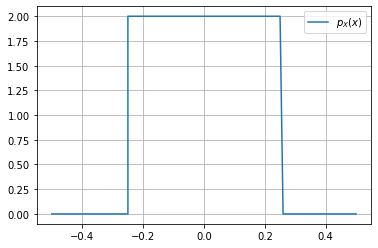
\includegraphics[width=\columnwidth]{Figure16_1}
\caption{PMF of $Y$}
\label{fig:pmf_x}	
\end{figure}

\numberwithin{figure}{section}
\begin{figure}[!ht]
\centering
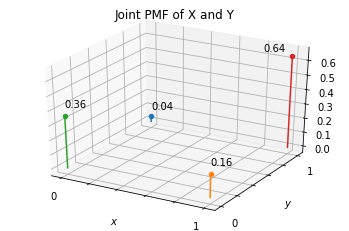
\includegraphics[width=\columnwidth]{Figure16_2}
\caption{Joint PMF of $X,Y$}
\label{fig:joint_pmf}	
\end{figure}

\end{document}

